%%
%% ArXiv paper 2401.09436 with markup enhanced for PDF/UA-2 compliant tagging
%%
\DocumentMetadata{
 lang=en,
 testphase={
     phase-III
    ,math,table,title
     },
 pdfversion=2.0,
 pdfstandard=ua-2,
 pdfstandard=a-4f,
 uncompress
 }
%\tagpdfsetup{math/mathml/write-dummy}

\documentclass[a4paper,11pt]{article}

%\usepackage[margin=1in]{geometry}
\usepackage[utf8]{inputenc}
\usepackage{
  %amsthm,
  amsmath,amssymb}
\usepackage{tikz}
\usepackage{graphicx,subcaption,caption}
\usepackage{algorithm,algorithmic}
\usepackage{pgfplots}
\usepackage{multirow}
\usepackage[T1]{fontenc}
%%%%%%%%%%%%%%%%%%%%%%%%%%%%%%
%% If your tex system is less than 2 years old (in 2012) the following
%% font options are available. If not comment them out.
\usepackage{tgtermes}
%       otherwise use alternative journal fonts
%\renewcommand{\rmdefault}{ptm} % system default Times font
\usepackage{mathptmx}  
%%%     additional fonts
\usepackage[scaled=.92]{helvet}
%\setoptfont{enc={T1},fam={pop}} % if You have Optima font, uncomment this line
%%% MATH
%\usepackage{amsthm,amsmath,amssymb}
\usepackage{mathrsfs}
%%% BIBLIOGRAPHY
%\usepackage{natbib}  %% numbers is required.
%%% LINKS
\usepackage[colorlinks,citecolor=blue,urlcolor=blue]{hyperref}  %%check

\usepackage{enumerate}

%\artstatus{am} %%% leave this alone!!  That means you, too!!
%%%%%%%%theorems%%%%%

%%%% feel free to changes these%%%%%%%
\newtheorem{theorem}{Theorem}[section]
\newtheorem{lemma}[theorem]{Lemma}
\newtheorem{problem}[theorem]{Problem}
\newtheorem{conjecture}[theorem]{Conjecture}
\newtheorem{condition}[theorem]{Condition}
\newtheorem{claim}[theorem]{Claim}
\newtheorem{question}[theorem]{Question}
\newtheorem{corollary}[theorem]{Corollary} 
%dpc\theoremstyle{definition}
\newtheorem{definition}[theorem]{Definition}
\newtheorem{statement}[theorem]{Statement}
\newtheorem{notation}[theorem]{Notation} 
% dpc\theoremstyle{remark}
\newtheorem{remark}[theorem]{Remark}
% dpc 
\newenvironment{proof}{\par\noindent\textbf{Proof}\par}{\par}
% dpc would need \ensuremath{\square} if luatex not used, but arxiv html does not use math
\newcommand\qed{\square}


%\tikzexternalize 
%\newtheorem{theorem}{Theorem}
%\newtheorem{proposition}{Proposition} 
%\newtheorem{lemma}{Lemma}
%\newtheorem{assumption}{Assumption}
%\newtheorem{remark}{Remark}
%\newtheorem{corollary}{Corollary}
%\newtheorem{definition}{Definition}
%\usepackage{hyperref}
%\providecommand{\keywords}[1]{\textbf{\textit{Keywords---}} #1}

%\firstpageno{1}

\begin{document}
%	\begin{frontmatter}
	\title{Computability of Approximate Optima of Nonconvex Functions}
	\author{K. Lakshmanan \\ Department of Computer Science and Engineering, \\ Indian Institute of Technology (BHU) Varanasi, 221005 India. \\ Email: lakshmanank.cse@iitbhu.ac.in}
	\date{}

	\maketitle
		
	\begin{abstract}
		It is known that finding approximate optima of non-convex functions is intractable. We give a simple proof to show that this problem is not even computable. \\ 
		\textbf{Keywords:}	Computablity of Approximate Optima, Non-convex functions
	\end{abstract}
	
	\section{Introduction and Preliminaries}
	We consider the problem of finding the global minima of a non-convex continuous function $f:  C \rightarrow \mathbb{R}$, where $ C \subset \mathbb{R}^d$ is a closed, compact subset. Global minima is the point $x^* \in C$ which satisfies the following property: $f(x^*) \leq f(x)$ for all $x \in C$. The function $f$ attains this minimum at least once by extreme value theorem. Our goal is to find one such point. This problem is well-studied with many books written on the subject, see for example \cite{globook}.

	We note that we consider an oracle setting, where the function values are given by an oracle. This is different from the computablity of optima computable real functions studied for example in \cite{pour}. It is easy to see that a simple grid search will output a sequence of points converging to the global optima. And for a Lipschitz continuous function, it requires an exponential number of oracle calls \cite{nest} if the Lipschitz constant is known. % that the approximations to optima are not computable too. %This is also the case if we are looking for points close to approximate optima.
	
	Let us define $S = \{x||f(x)-f(x^*)|\leq \epsilon\}$ and term the members of $S$ as $\epsilon$-optima. In optimization literature \cite{foster2019complexity,zhang2020complexity}, it is known that finding approximations to optima is not tractable for non-convex functions. For non-convex functions, $\epsilon$-stationary point which is weaker than $\epsilon$-optima is also known to be not tractable \cite{zhang2020complexity}. We show more in this paper, that this set $S$ is not computable. This is much stronger than saying they it is intractable. We assume for formality finite-precision numbers. This assumption of finite-precision numbers is useful to model real-world systems and we show is not restrictive.
	
	%and $T = \{y|\exists x \mbox{ s.t., } |x-y| \leq \delta \mbox{ and } |f(x)-f(x^*)|\leq \epsilon \}$.
	% and that of $T$ as $(\epsilon,\epsilon)$-optima.
	 %Our proof is through simple reductions.
	
	%\begin{table}[ht]\label{table1}
	%	\centering
	%	\begin{tabular}{|p{4cm}|c c|} 
	%		\hline
	%		\multirow{2}{*}{Function Type} & \multicolumn{2}{c}{Function Oracle} \\
	%		& Yes & No \\
	%		\hline
	%		Computable-Real & No & No \\
	%		Computable-Real (Isolated minimum) & \multirow{2}{*}{Yes} & \multirow{2}{*}{Yes}\\
	%		Lipschitz Continuous & Yes & No \\
	%		Differentiable/Smooth & No & No \\
	%		Continuous & No & No \\
	%		\hline
	%	\end{tabular}
	%	\caption{Computable Convergence to Global Minimum }
	%	\label{tab1}
	%\end{table}
	
	\subsection{Finite Precision Reals}
	We now briefly explain what we mean by this.
	Consider any real number $x \in \mathbb{R}$. Let $r_0$ be the largest integer such that $r_0 \leq x$. Having chosen $r_0,r_1,\ldots,r_{k-1}$ choose largest positive integer $r_k$ such that
	\[ r_0 + \frac{r_1}{10} + \frac{r_2}{10^2} + \ldots \frac{r_k}{10^k} \leq x. \]
	
	This is the decimal expansion of the number. We can check that this expansion is unique. We define precision length to be the number $k$.
	Now for finite precision representaion of a real we need to specify this precision length $k$. And we say for any real $x \in \mathbb{R}$, the numbers $r_0,r_1,\ldots,r_k$ is its finite precision representation. Note that $r_i, 0\leq i \leq k$ can be zero.  %We can consider this finite-precision real number as a natural number by representing it as $r_0*10^k+r_1*10^{k-1}+\ldots+r_k$. For $x \in \mathbb{R}^d$,%all finite-precision lengths of its coordinates.
	For a point $x \in \mathbb{R}^d$, given a precision length $k$ we can have decimal expansions for all it's co-ordinates.
	Note that though we give binary representations to the Turing machine, for simplicity we assume precisions denote the decimal precisions.
	
	\begin{remark}\label{gaprem}
		Suppose $r_1,\ldots,r_k$ is the finite precision representation with length $k$ of some real $x$. Let $\bar x$ be the number with decimal expansion $r_1,\ldots,r_k$ as $x$ and $r_{l}=9$ for $l \geq k+1$. And let $\underline x$ be the number with decimal expansion $r_1,\ldots,r_k$ as $x$ and $r_{l}=0$ for $l \geq k+1$. %We can see that for all reals in $[\underline x,\bar x]$ we have the same finite length representation. 
		And the length of this interval $[\underline x,\bar x]$ is $\epsilon = 10^{-k}$. We then say with precision length $k$ we can represent consecutive numbers with gap greater than or equal to $\epsilon$.
	\end{remark}
	
	\subsection{The Problem}
	We assume there is an oracle for our continuous function $f$. This oracle gives the value $f(x)$ up to any finite-precision for an given finite-precision $x$. The Turing-machine has access to this function oracle. We give also give a value $\epsilon > 0$ as input to the Turing machine. Our main problem is to write any point $x_{o}$ of the finite precision length such that $|f(x_{o})-f(x*)| < \epsilon$ i.e., it should find $\epsilon-$ approximation of the global optima. We show that this problem is not computable.
	
	Let us assume we have a three-tape Turing machine, one is used for calculations, second is for the giving the finite precision real and the precision length required to the function oracle and third one has the value returned from the oracle \cite{sorbook}. Note that the third tape can also store the previous values. That is suppose we start with $x_0$ and find $x_1,\ldots,x_{k}$ this tape can store all these and also the corresponding function values obtained from the function oracle $f(x_0),\ldots,f(x_k)$ for finding $x_{k+1}$. We now give definition of the standard Turing machine here:
	
	\begin{definition}
		Turing machine has a three infinite tapes divided into cells, a reading head which scans one cell of the tape at a time, and a finite set of internal states $Q=\{q_0,q_1,\ldots,q_n\}, \, n \geq 1$. Each cell is either blank or has symbol 1 written on it. In a single step the machine may simultaneously (1) change the from one state to another; (2) change the scanned symbol $s$ to another symbol $s'\in S = \{1,B\}$; (3) move the reading head one cell to the right (R) or left (L). This operation of machine is controlled by a partial map $\Gamma : Q \times S^3 \rightarrow Q \times (S \times \{R,L\})^3$.
	\end{definition}
	
	\begin{remark}
		The map $\Gamma$ viewed as a finite set of quintuples is called a Turing program. The interpretation is that if $(q,s_1,s_2,s_3,q',s'_1,X_1,s'_2,X_2,s'_3,X_3) \in \Gamma$, in state $q$, scanning symbols $s_1, s_2, s_3$ changes state to $q'$ and in the tape $i$ input symbol to $s'_i$ and moves to scan one square to the right if $X_i=R$ (or left if $X_i=L$.) in the tape $i$.	
	\end{remark}
	
	We consider this problem in the paper.
	
	\begin{problem}
		Given a continuous, nonconvex function $f$, is there a Turing machine with access to the function oracle which can find a $\epsilon-$ approximation to the global optima of the function $f$ ?
	\end{problem}
	
	\section{Main Theorem}
	
	%Given a input $x$ of finite precision length $n$, the oracle can return $f(x)$ to any specified precision.
	Given the objective function $f$, let the set of global minima be denoted by $G^f$. Now consider $\epsilon$-approximation to the global minima.  %We consider finite length approximation of the set $G'_{\epsilon}$. 
	
	\begin{lemma}\label{preclem}
		For all $\epsilon > 0$ there exists a point $x_n^*$ of finite precision length $n$ such that $|f(x^*)-f(x_n^*)| < \epsilon$. 
	\end{lemma}
	
	\begin{proof}
		Let $\delta > 0$ be such that $|x-y| < \delta$ implies $|f(x)-f(y)| < \epsilon$. Such an $\delta > 0$ exists for all $\epsilon > 0$ because the function $f$ is continuous. Let $n$ be the precision length required to represent numbers with gap $\epsilon/10$ between consecutive numbers (Remark \ref{gaprem}). Then we see for the global minima $x^*$ (like for all other points) it's finite precision representation $x_n^*$ with precision length $n$ is such that $|x_n^*-x^*|<\epsilon$. 
	\end{proof}
	
	\begin{definition}
		Let $G^f_{\epsilon,k}$ be the set of points with given finite precision length $k \geq 1$ where the function value is $\epsilon > 0$ close to the global minima. And $G^f_{\epsilon}$ be the union of all such sets.
	\end{definition} % We show that this set $G'_{\epsilon}$ is not limit computable.
	We consider only finite-precision numbers. %As the domain is a compact set, this can be regarded as a subset of natural numbers by multiplying by an appropriate constant. And in particular
	As there are only finite number of points with precision length $k$, the set $G^f_{\epsilon,k}$ is finite. 
	Since we would like an algorithm to computably converge to a single point, for simplicity we assume the global optima is unique i.e., $G^f$ is a singleton. This is not uncommon in optimization literature as strict convexity gives unique local (global) minima and is assumed for objective functions. Now we state the main theorem.
	
	\begin{lemma}\label{checklem}
		There is no algorithm to check if a point $x_k$ is a $\epsilon-$ approximation  to the global optima.
	\end{lemma}
	
	\begin{proof}				
		We consider an equivalent problem. We define
		\begin{equation*}
			h_{x_k}^{\epsilon}(x) := \max \{0,f(x_k)-f(x)-\epsilon\}.
		\end{equation*}
		Since our objective function $f$ is continuous, $h_{x_k}^{\epsilon}(\cdot)$ is also continuous. 
		This function is identically zero if and only if $|f(x_k) - f(x)| < \epsilon$, for all $x$. This happens only if $x_k$ is a $\epsilon-$ approximation to the optimum (See Figure \ref{illusfig}). Note that $x_k$ and $x$ are represented with some finite precision. % then $h_{x_k}^{\epsilon}(\cdot)$ is identically zero. %Or to find a finite-precision point $y$ which is $\epsilon-$ approximation to the optimum is same as finding a function $h_y^{\epsilon}(\cdot)$ which is identically zero for some $y$. But this cannot be checked for any particular value of $y$.
		\begin{figure}[!ht]
			\centering
%dpc add alt
			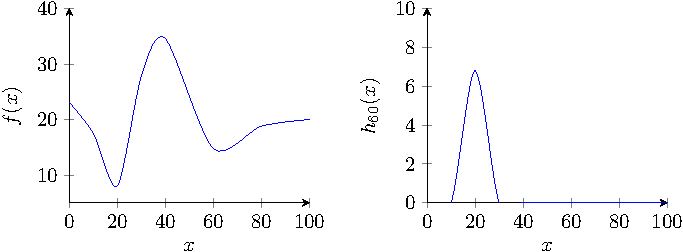
\includegraphics[alt={Two plots of function graphs}]{fig1-crop.pdf}
			\caption{The figure on the right shows a sample objective function. The figure of the left is the function $ \max \{0,f(60)-f(x) \}$. This function  is not identically zero as $x=60$ is not the global minima of $f(x)$.}
			\label{illusfig}
		\end{figure}
		
		
		Thus the set $G^f_{\epsilon}$ of all points with finite precision that are $\epsilon$ close to the global minima, is precisely the set of all points $x_k$ where the function $h_{x_k}^{\epsilon}(\cdot)$ is identically zero.
		That is, 
		\[ x_k \in G^f_{\epsilon} \Leftrightarrow h_{x_k}^{\epsilon}(x) = 0 \mbox{ for all } x \in C \]
		But this cannot be checked for a particular $x_k$ unless it is checked for all $x$ of any finite precision length. As there are infinitely many such points, there is no Turing machine which can compute (halt) if a function is zero at infinitely many points.
		So given any point $x_k$, it is not possible to say if it is an $\epsilon-$ approximation to the global optima or not.
		\end{proof}
		
		\begin{theorem}\label{mainthm}
			We assume the objective function we wish to minimize is known by its oracle. There is no algorithm which can compute the $\epsilon$-approximate optima of a continuous, non-convex objective function on a compact domain.
		\end{theorem}
		
		\begin{proof}
		Let $x'_k$ be any point of some finite precision length $n_k$ such that $|f(x^*)-f(x'_k)| < \epsilon$. Such a point exists by Lemma \ref{preclem} i.e., the set $G^f_{\epsilon,n_k}$ is non-empty for $\epsilon > 0$. Suppose that we have an algorithm to find a $\epsilon/2-$ approximation point $x'_k$.% This length $n_k$ can increase with $k$.

		Now for any point $x_k \in C$ we can say it is $\epsilon$ close to optimum if $|f(x_k)-f(x'_k)| < \epsilon/2$ else it is not. Thus we have an algorithm to check if a point is an $\epsilon-$ approximation to the global optima or not. This is a contradiction to Lemma \ref{checklem}. Thus for a $\epsilon > 0$, there is no algorithm to find a $\epsilon-$ approximation to the global optima. 
		
		%we can not compute any $N$ such that for all $n \geq N$ with $\{x_n\}$ having finite precision, $|f(x_n) - f(x^*)| < \epsilon$.
		%In other words, we see that there is no computable sequence with finite precision length $\{ x_k \}$ converging to the global optimum (Definition \ref{ccdef}). Thus we have shown the theorem.
		%there is no sequence of computable $\{x_k\}$ with finite-precision length converging to the global minima.
	\end{proof}
	
	\begin{corollary}
		The finite-precision assumption is not restrictive. If there is an algorithm to find a general real number which is $\epsilon-$ approximation, we can take the first $k$ digits which gives $\epsilon-$ approximation to get a finite precision approximation. %If an algorithm outputs real vectors $\{x_k\}$ converging to the global minimum, then by taking the first $k$ digits of each co-ordinate in $x_k$ it can output a sequence of real vectors with finite-precision length converging to the same point. By contra-positive, if there is no algorithm which can output finite-precision points then there can be no algorithm which outputs any sequence of points converging to the global minimum.
	\end{corollary}
	
	%\begin{corollary}
	%	The problem of approximating the global minima of a continuous function by an arbitrary $\epsilon > 0$ is not computable.
	%\end{corollary}
	
	\begin{corollary}
		The problem of checking whether local minima $z$ is global is not computable as this also involves checking whether $h_z^{\epsilon}(\cdot)$ is identically zero.
	\end{corollary}
	
	\begin{remark}
		Even in presence of higher order oracles, i.,e oracles which give derivatives of the function, the equivalent problem of checking if $h_z^{\epsilon}(\cdot)$ is identically zero remains. Hence global optima even in presence of these higher-order function oracle is not computable. %(\#\#\# if bound on gradient is not known \~ Lipschitz)
	\end{remark}
	
	\begin{remark}
		As we mentioned before, our result is for algorithms having access to the function oracle. This is different from the setting of computable function and reals studied in computable analysis. \cite{pour}
	\end{remark}
	
	\begin{remark}
		As we can find an ball of some radius $\omega$ where the continuous function $h_z^{\epsilon}(\cdot)$ is non-zero around a local optima. The same proof does not hold for converging to local optima as we can check if $h_z^{\epsilon}(\cdot)$ is identically zero in steps of size less than $\omega$.
	\end{remark}
	
	\section{Global Optima Property}
	In this section, we see a simple property a function satisfies if the global optima is computable. For this let us first define the set $G^f$ of global optima of the function $f:C\rightarrow \mathbb{R}$, $C\subset \mathbb{R}^d$ as
	\[ G^f := \{x\,| \, \mbox{ for all } y, \, f(x) \leq f(y), \, x \in C \}.\]
	
	This set $G^f$ is a subset of $C$. As we are interested in finding only one optima, we call $G^f$ computable if atleast one of it's member is. %We now claim that if the global optima is computable then function must satisfy a property of a particular form.
	
	\begin{definition}
		A function $f$ satisfies global property if there is a first order (3-ary) predicate $P_{\zeta}(y,x)$ and a $\zeta \in \mathbb{R}$ such that $P_{\zeta}(y,x)$ is True for all $y,x$ in the domain $C$ of the function $f$.
	\end{definition}
	
	We say a property $P_{\zeta}(y,x)$ can be computed if $\zeta$ in the definition can be computed.
	
	\begin{definition}
		A set of functions $\mathcal{F}$ satisfies a global property if there is a first order predicate $P_{\zeta}(y,x)$ satisfied by all the functions $\mathcal{F}$.%  such that the predicate is True for all $y, x$ in the domain $C$ of the function $f$.
	\end{definition}
	
	%We represent True by 1 and False by 0. For example if we let
	%We can see that this property $Q^f_{x^*}(y)$ defines the global minima and is satisfied by all continuous functions on compact domain.
	
	%\begin{theorem}[Global Optima Property]
	%	There is a algorithm to converge to the global optima of a set of functions $\mathcal{F}$ if and only if there exists a computable global property $P_{\zeta} (y,x)$ that is satisfied by all the functions in $\mathcal{F}$.% for some computable $\zeta \in \mathbb{R}$. %satisfies the property $P_\zeta (y,x)$.% for all $y$ and $x$ in the domain $C$. Note that here the property $P^f_\zeta (y,x)$ need to be satisfied for all $x \in C$ not just the set $G^f$ of global optima.
	%\end{theorem}
	
	\begin{remark}
		%Here we assume we are finding minima. There could be more than one global minima and we need to find one.
		If the global minima is computable for a function $f$, we can easily define the $\zeta$ to be the norm of a member of $G^f$ which is computable, say $x^*$ and the global property to be 
		\[ P_{\zeta}(y,x) \mbox{ is True for all } x, \, y \mbox{ if there exists a } x \mbox{ s.t. } \parallel x \parallel = \zeta.\]
		%\begin{table}[h]
		%	\centering
		%	\begin{tabular}{cl} 
		%		\multirow{2}{1.4cm}{$P^f_{\zeta}(y,x) =$} &1 if $\parallel x \parallel = \zeta$ \\ %, \mbox{for some } x^* \in G^f, $ \\ 
		%		&0 o.w.
		%	\end{tabular}
		%\end{table}
		It is clear that if global optima is computable then this $P_{\parallel x^* \parallel}(y,x)$ is satisfied by the function $f$ and $\parallel x^* \parallel$ can be computed.
		
		%Now for the other direction, assume that global minima is not computable. But there is some property $P_{\zeta}(y,x)$ where one can find a computable $\zeta \in \mathbb{R}$ such that the property is satisfied by the function $f$. Now we look at the definition of global minima and define another global property for $f$ as 
		
		%\[P_{\zeta}(y,x) \mbox{ is True for all } x, y, \zeta \mbox{ if there exists a } x \mbox{ s.t. for all } y, f(x) \leq f(y). \]
		
		%\begin{table}[h]
		%	\centering
		%	\begin{tabular}{cl} 
		%		\multirow{2}{1.1cm}{$P^f_{\varepsilon}(y,x)=$} & 1 if $f(x) \leq f(y), \forall y$ \\ 
		%		&0 o.w.
		%	\end{tabular}
		%\end{table}
		
		%And by assumption we can not find a computable $\zeta$, such that $P_{\zeta}(y,x)$ is satisfied by $f$. But this is a contradiction to the existence of global optima $x^*$, as $P_{\zeta}(y,x^*)$ is satisfied by $f$ for all $\zeta$ and this property can be computed if $x^*$ is computable. Thus we have shown the structure of the global property which must be satisfied for the global optima to be computable.
		%independent of the value of $\varepsilon$
	\end{remark}
	
	\begin{remark}
		Lipschitz continuity is another example of such a global property. Let $P_L(y,x)$ be 
		\[|f(x)-f(y)| \leq L \parallel x - y \parallel, \, \mbox{ for all } x,y \, \in C.\]
		And here the number $\zeta$ is the Lipschitz constant $L$. Let the set of functions on some compact domain $C$ satisfying the Lipschitz property be denoted by $\mathcal{L}$. It is known that if the Lipschitz constant or an upper bound to it is known then the global optima for this class of functions $\mathcal{L}$ is computable. (For example refer to Theorem 1.1.2 of \cite{nest}). Another example of a global property is bounded derivatives. If a bound on the gradient is known then the global minima can be computed.
	\end{remark}
	
	\section{Conclusion}
	We have proved that there is no algorithm which finds a $\epsilon-$ approximation to the optima of nonconvex function $f$. This result holds even if the function has higher-order derivatives.
	
	\bibliographystyle{plain}
%	\bibliography{glosuba}
\begin{thebibliography}{1}

\bibitem{foster2019complexity}
Dylan~J Foster, Ayush Sekhari, Ohad Shamir, Nathan Srebro, Karthik Sridharan,
  and Blake Woodworth.
\newblock The complexity of making the gradient small in stochastic convex
  optimization.
\newblock In {\em Conference on Learning Theory}, pages 1319--1345. PMLR, 2019.

\bibitem{globook}
R.~Horst and H.~Tuy.
\newblock {\em Global Optimization: Deterministic Approaches}.
\newblock Springer-Verlag.

\bibitem{nest}
Y.~Nesterov.
\newblock {\em Introductory Lectures on Convex Optimization A Basic Course}.
\newblock Kluwer Academic Publishers.

\bibitem{pour}
M.~Pour-El and J.~Richards.
\newblock {\em Computability in analysis and physics}.
\newblock Springer, Heidelberg, 1989.

\bibitem{sorbook}
R.I. Soare.
\newblock {\em Turing Computability: Theory and Applications}.
\newblock Springer-Verlag.

\bibitem{zhang2020complexity}
Jingzhao Zhang, Hongzhou Lin, Stefanie Jegelka, Suvrit Sra, and Ali Jadbabaie.
\newblock Complexity of finding stationary points of nonconvex nonsmooth
  functions.
\newblock In {\em International Conference on Machine Learning}, pages
  11173--11182. PMLR, 2020.

\end{thebibliography}
	
\end{document}
